% !TEX root = main.tex

We present the results of the LCA analysis in relation to the 1) Embodied GWP, 2) a calculation of the emission factor, 3) global distribution of GWP, 4) regional effects of terrestrial acidification, 5) sensitivity of the LCA to design and location, and 6) a comparison to other PV technologies.

\subsection{LCA of the Adaptive Solar Facade Manufacture}

A breakdown of the embodied carbon emissions can be found in Figure  \ref{fig:embodied}. The largest embodied global warming potential (GWP) contribution in the ASF comes from the solar panels, the electronics and the supporting structure.

\begin{figure}[H]
\begin{center}
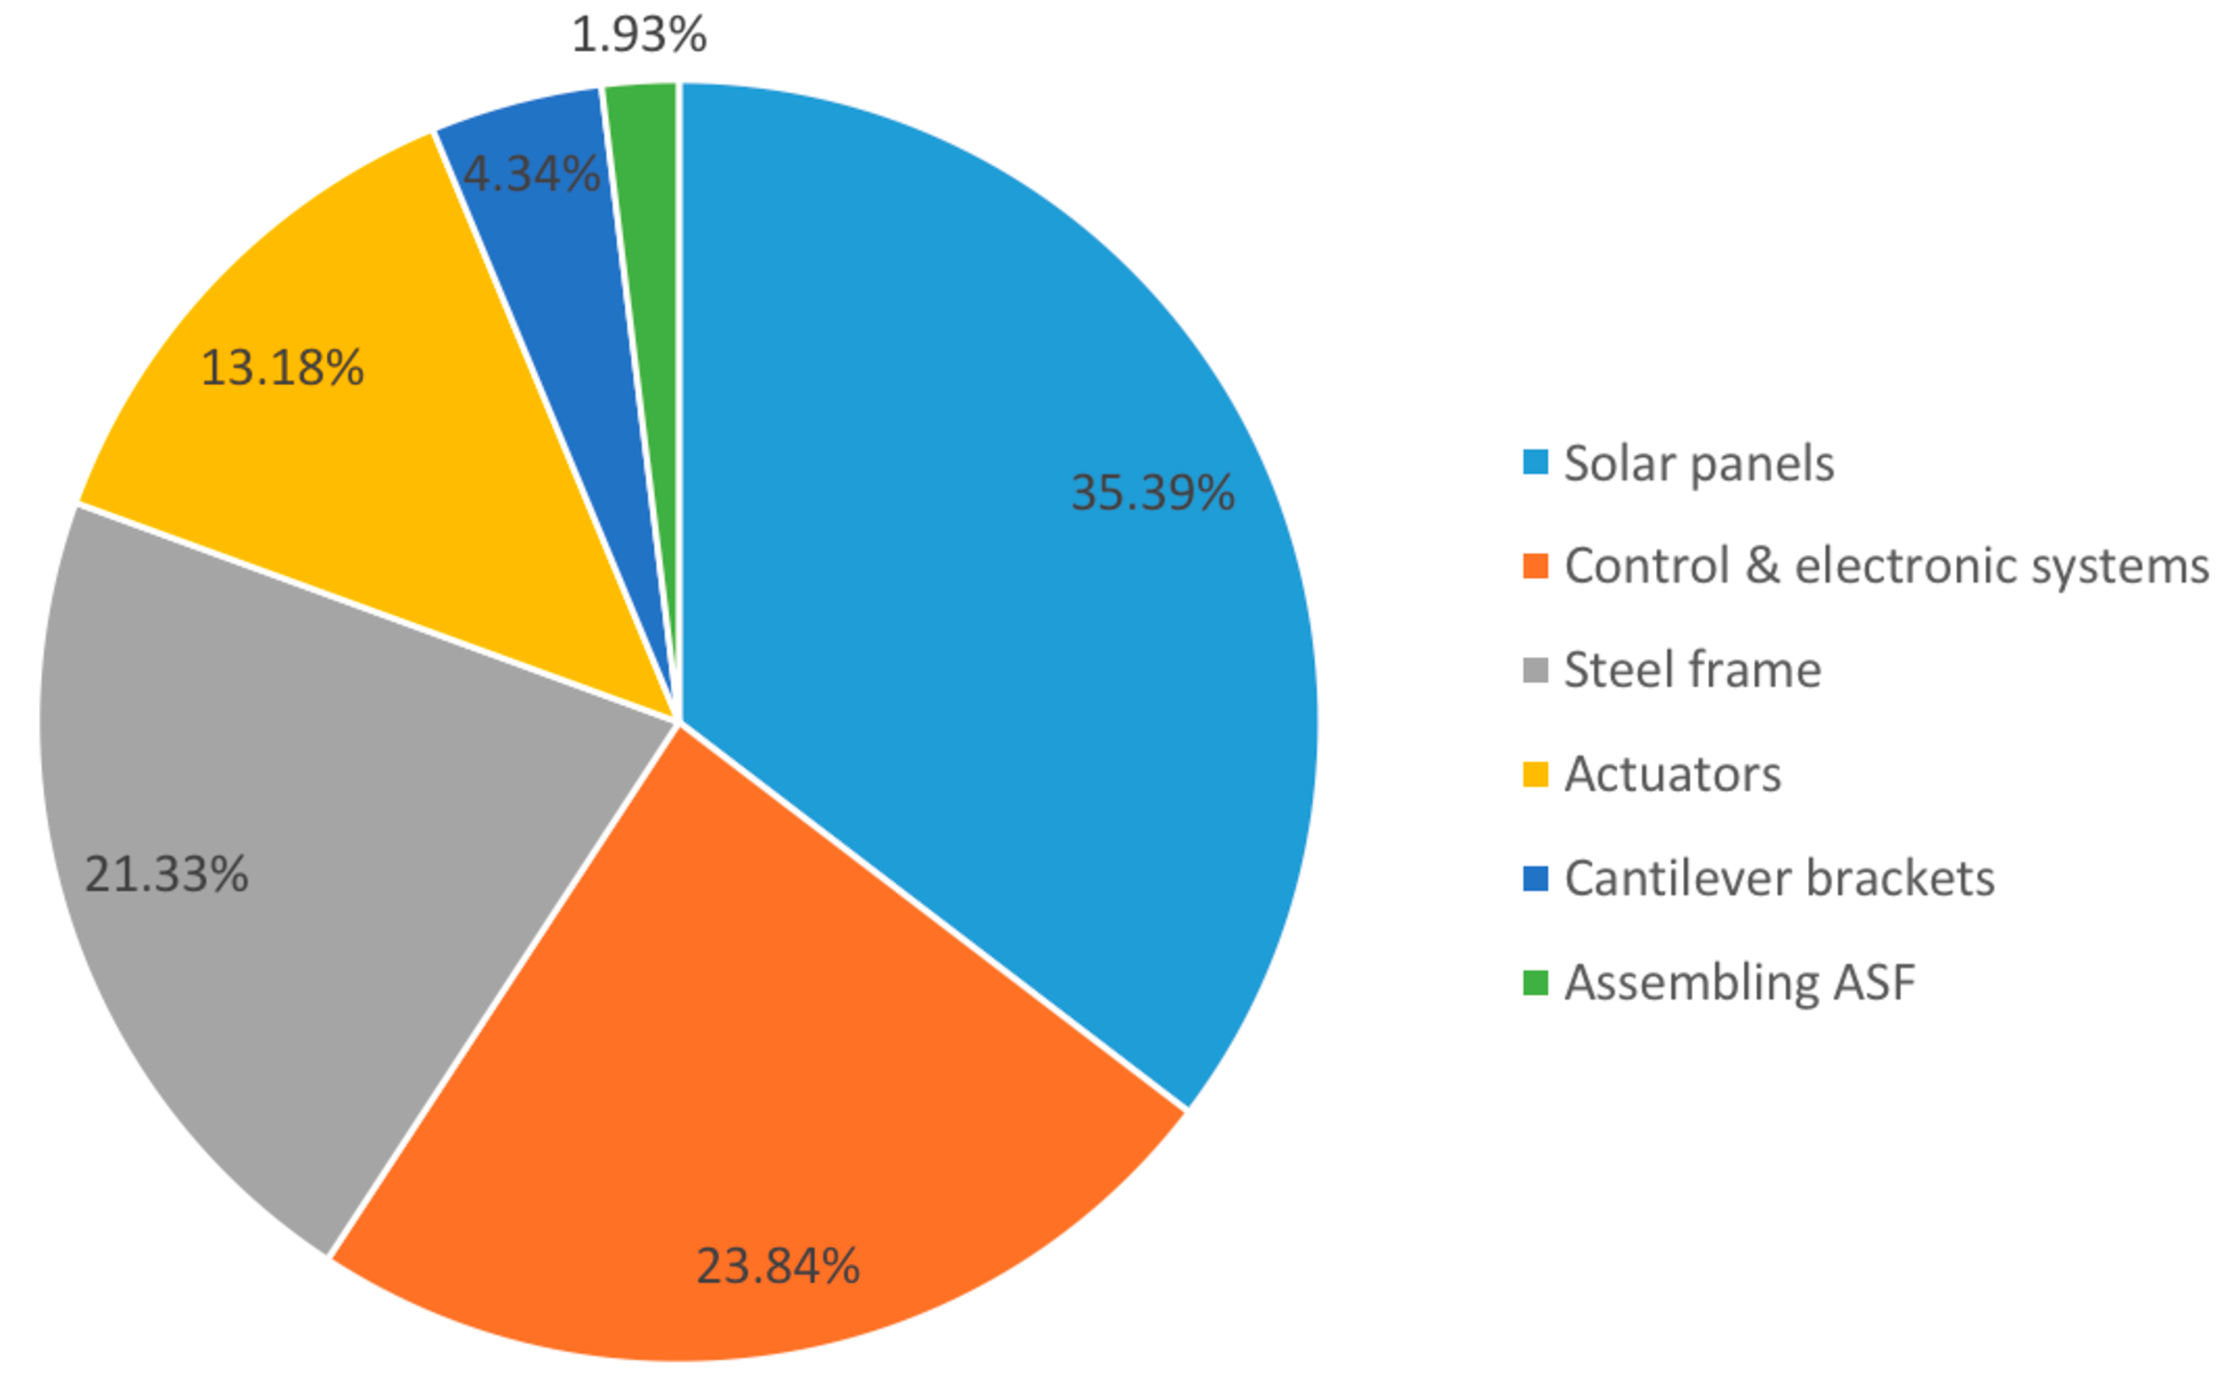
\includegraphics[width=10cm, trim= 0cm 0cm 0cm 0cm,clip]{pieembodied}
\caption{Breakdown of greenhouse gas emissions due to material production. The total is GWP is 2676.5 kg CO$_{2eq}$.}
\label{fig:embodied}
\end{center}
\end{figure}

\subsection{Calculation of Emission Factor}
The combined GWP of main inputs to the ASF, previously described in Figure \ref{fig:BOS}, can be built up using a waterfall chart as shown in Figure \ref{fig:waterfall}. 

This gives us a total GWP of -6229.6 kg CO$_{2eq}$. We calculate a total electricity production of 580kWh per year, resulting in an emission factor of -537.0 gCO${_2}$/kWh.

\begin{figure}[H]
\begin{center}
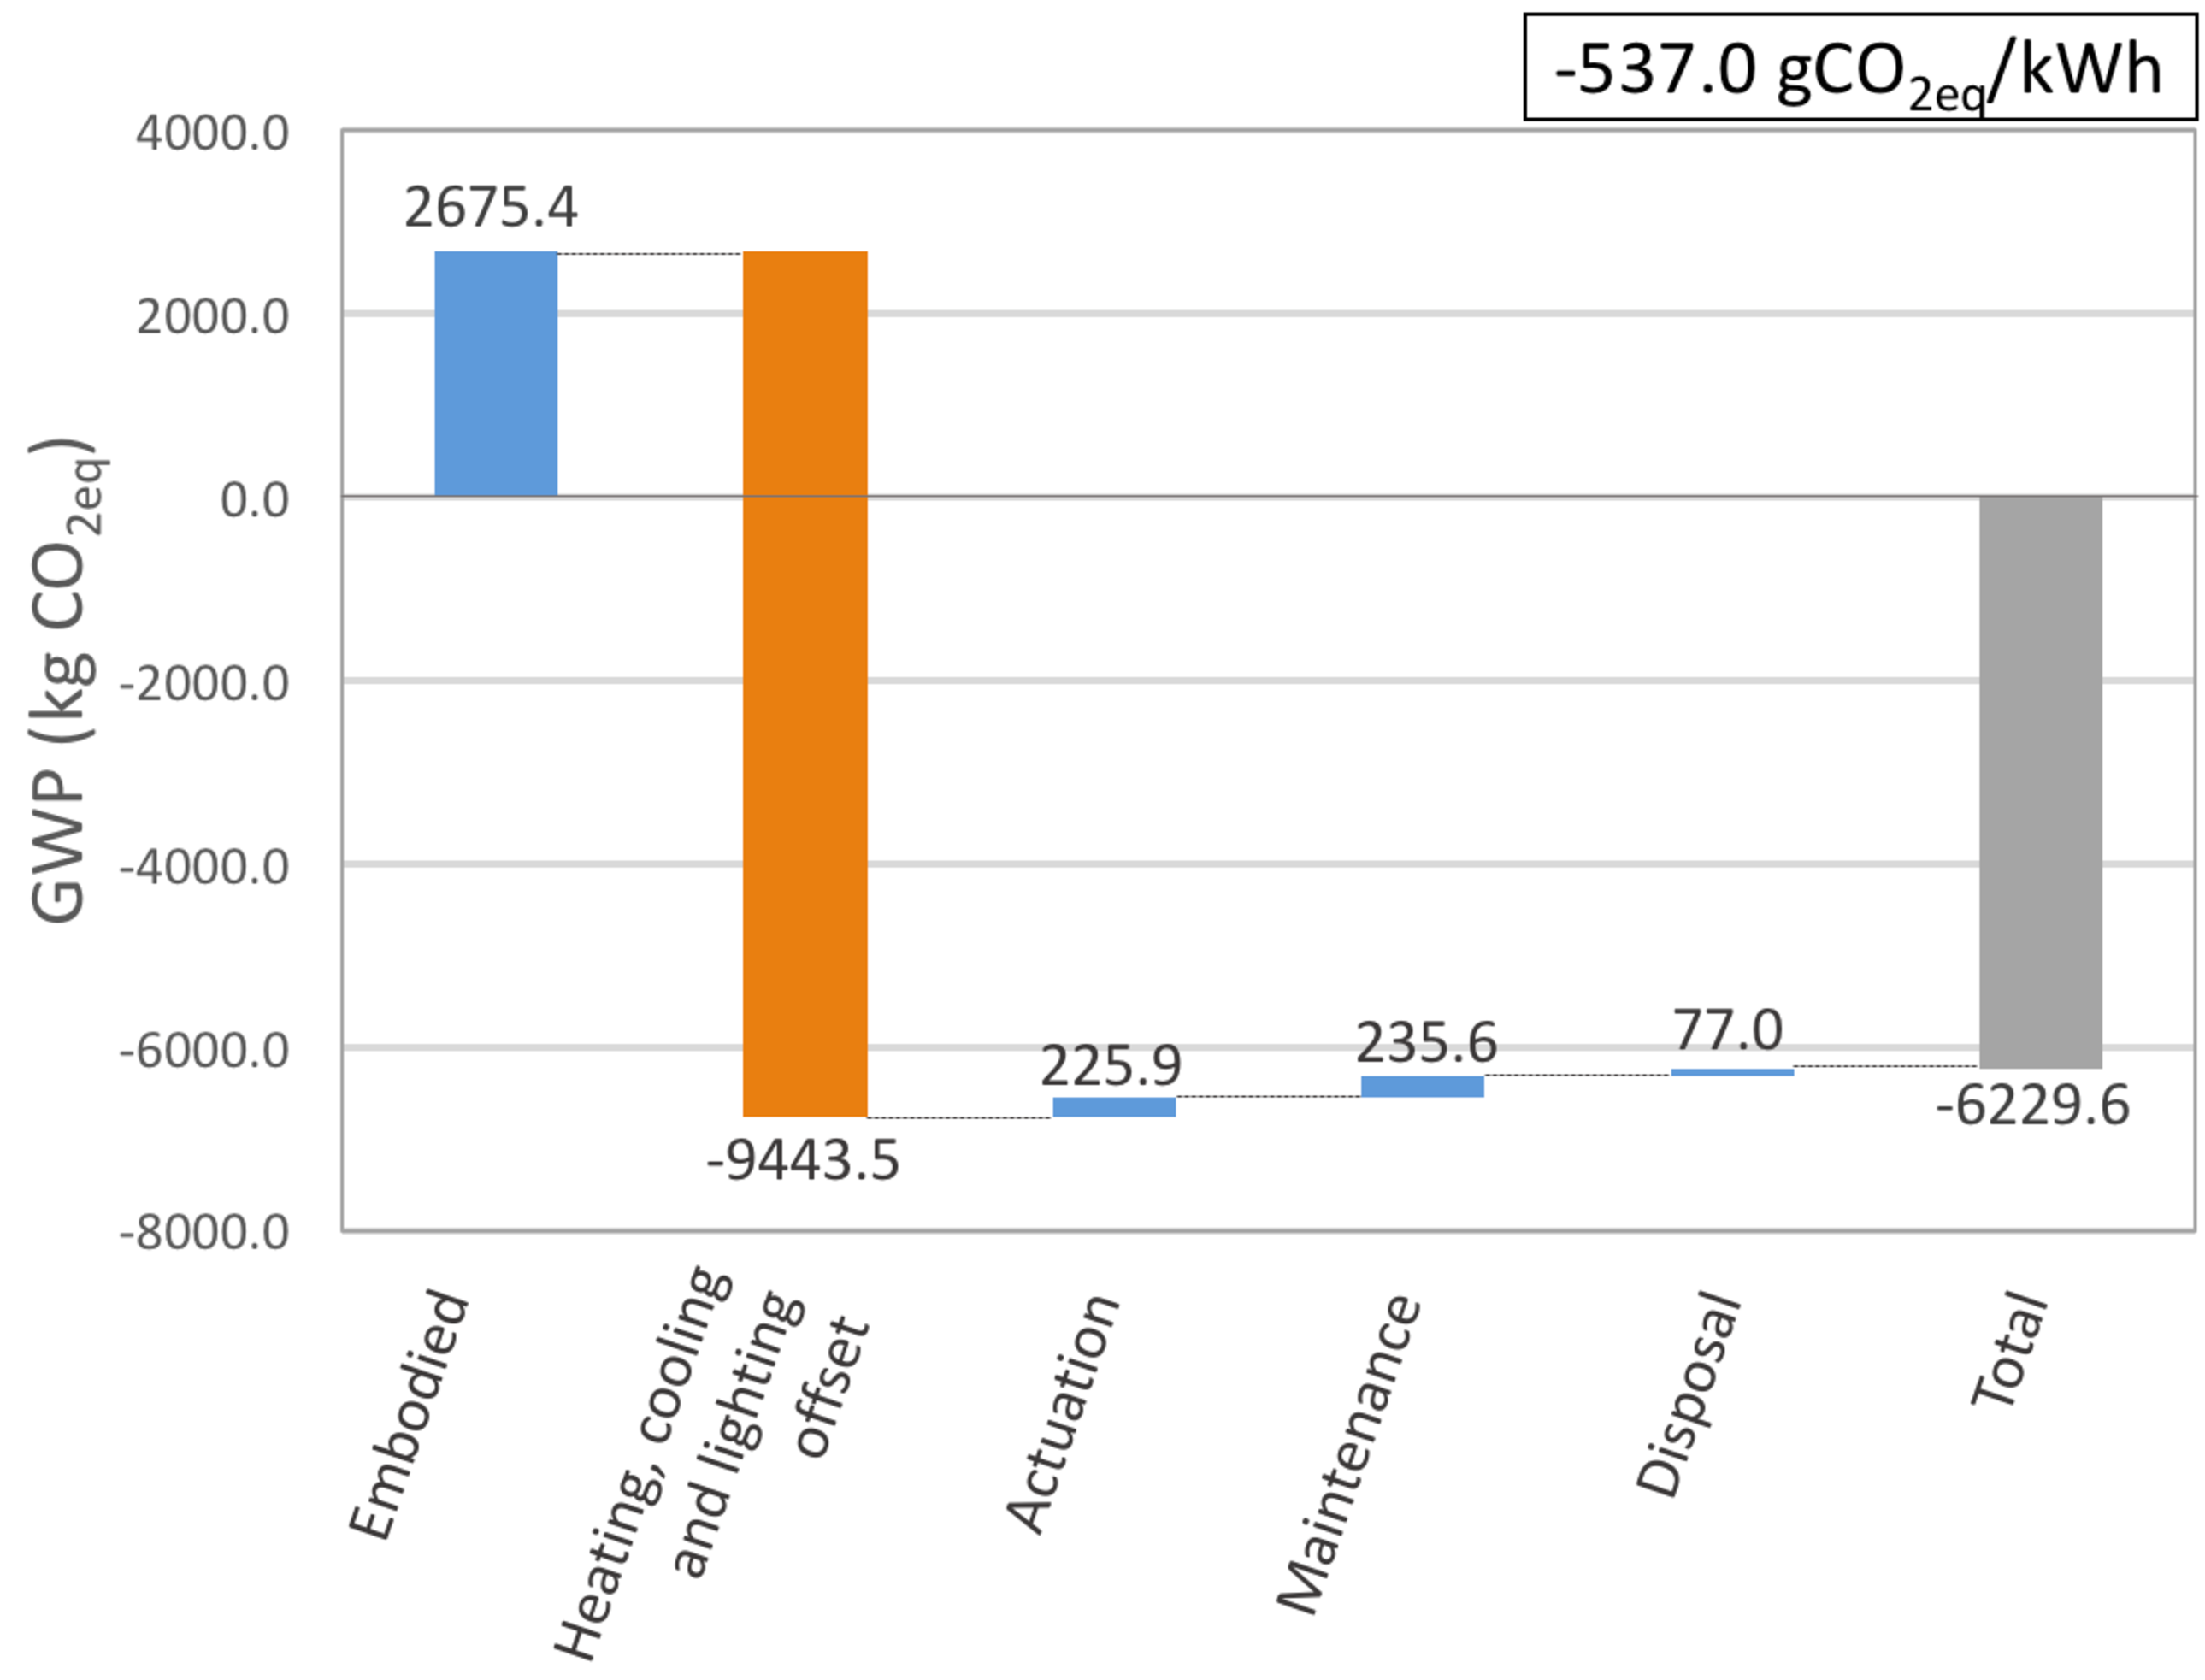
\includegraphics[width=12cm, trim= 0cm 0cm 0cm 0cm,clip]{waterfall}
\caption{Waterfall diagram of GWP of the ASF. The far left bar details the embodied carbon emissions. The second bar details the emission reduction of the building through the smart shading algorithms of the ASF. The third, fourth and fifth bar shows the effect of dynamic actuation, maintenance, and disposal respectively. This leaves us with a final emissions value (grey bar). When we apply this value to Equation \ref{eq:EF}, we obtain an emission factor per kWh of -537.0 gCO$_2$-eq./kWh.}

\label{fig:waterfall}
\end{center}
\end{figure}

\subsection{Global Distribution of GWP and Terrestrial Acidification}
%\textcolor{magenta}{\textit{I still think this is adding noise rather than useful information for a reader interested in BIPV. Plus I question the correctness of these figures. I would \textbf{only} keep this section if you draw meaningful conclusions from it. If you need references on regionalized LCIA (e.g. for the discussion), let me know... This is the only time you talk about acidification. You would need to justify that too.}}

The global distribution of embodied GWP emissions is focused in Europe, specifically Germany and Switzerland as most of the manufacturing is done in this region. It can be see however that emissions occur globally due the sourcing of primary materials from many locations around the world. Terrestrial acidification however is more interesting as it has a local impact compared to carbon emissions. It is interesting to note that China carries the greatest burden of terrestrial acidification from the ASF production.
 
\begin{figure}[H]
\begin{center}
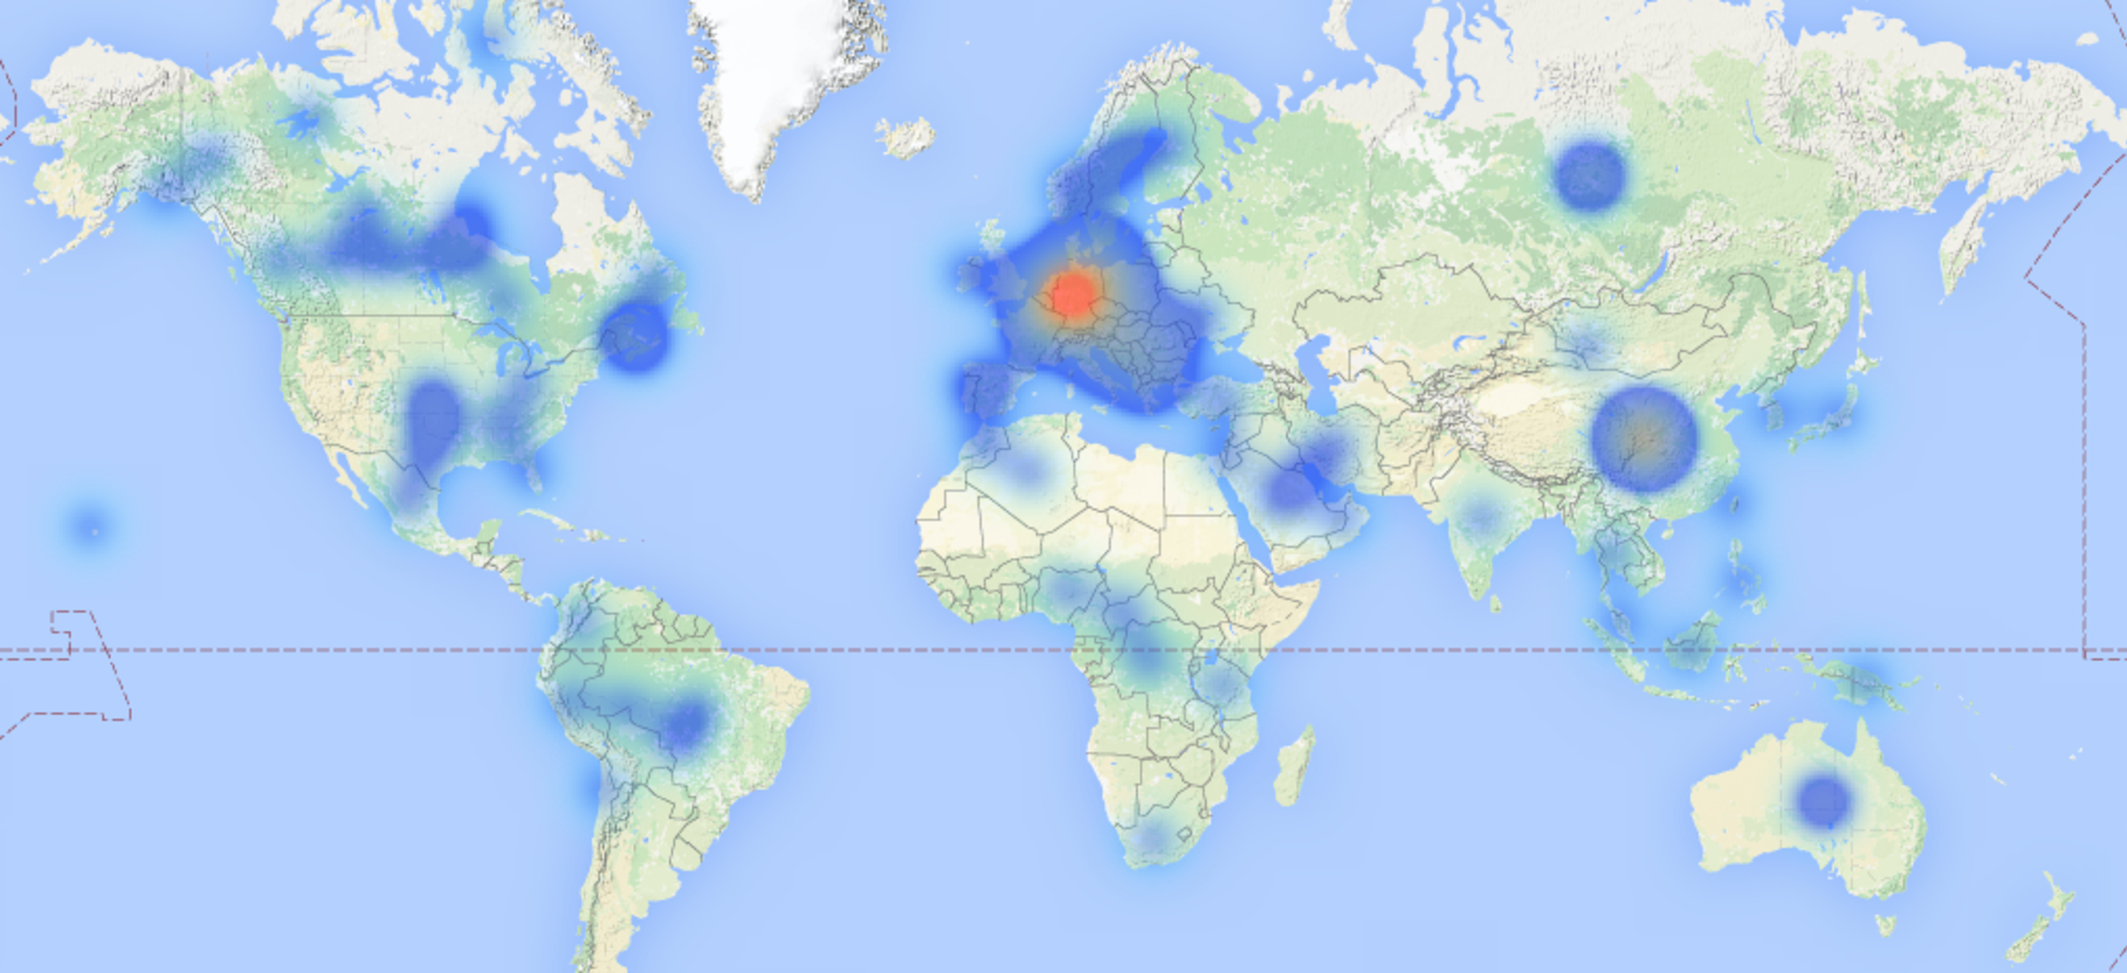
\includegraphics[width=10cm, trim= 0cm 0cm 0cm 0cm,clip]{mapGWP.pdf}
\caption{Global distribution of embodied GWP emissions}
\label{fig:mapGWP}
\end{center}
\end{figure}

\begin{figure}[H]
\begin{center}
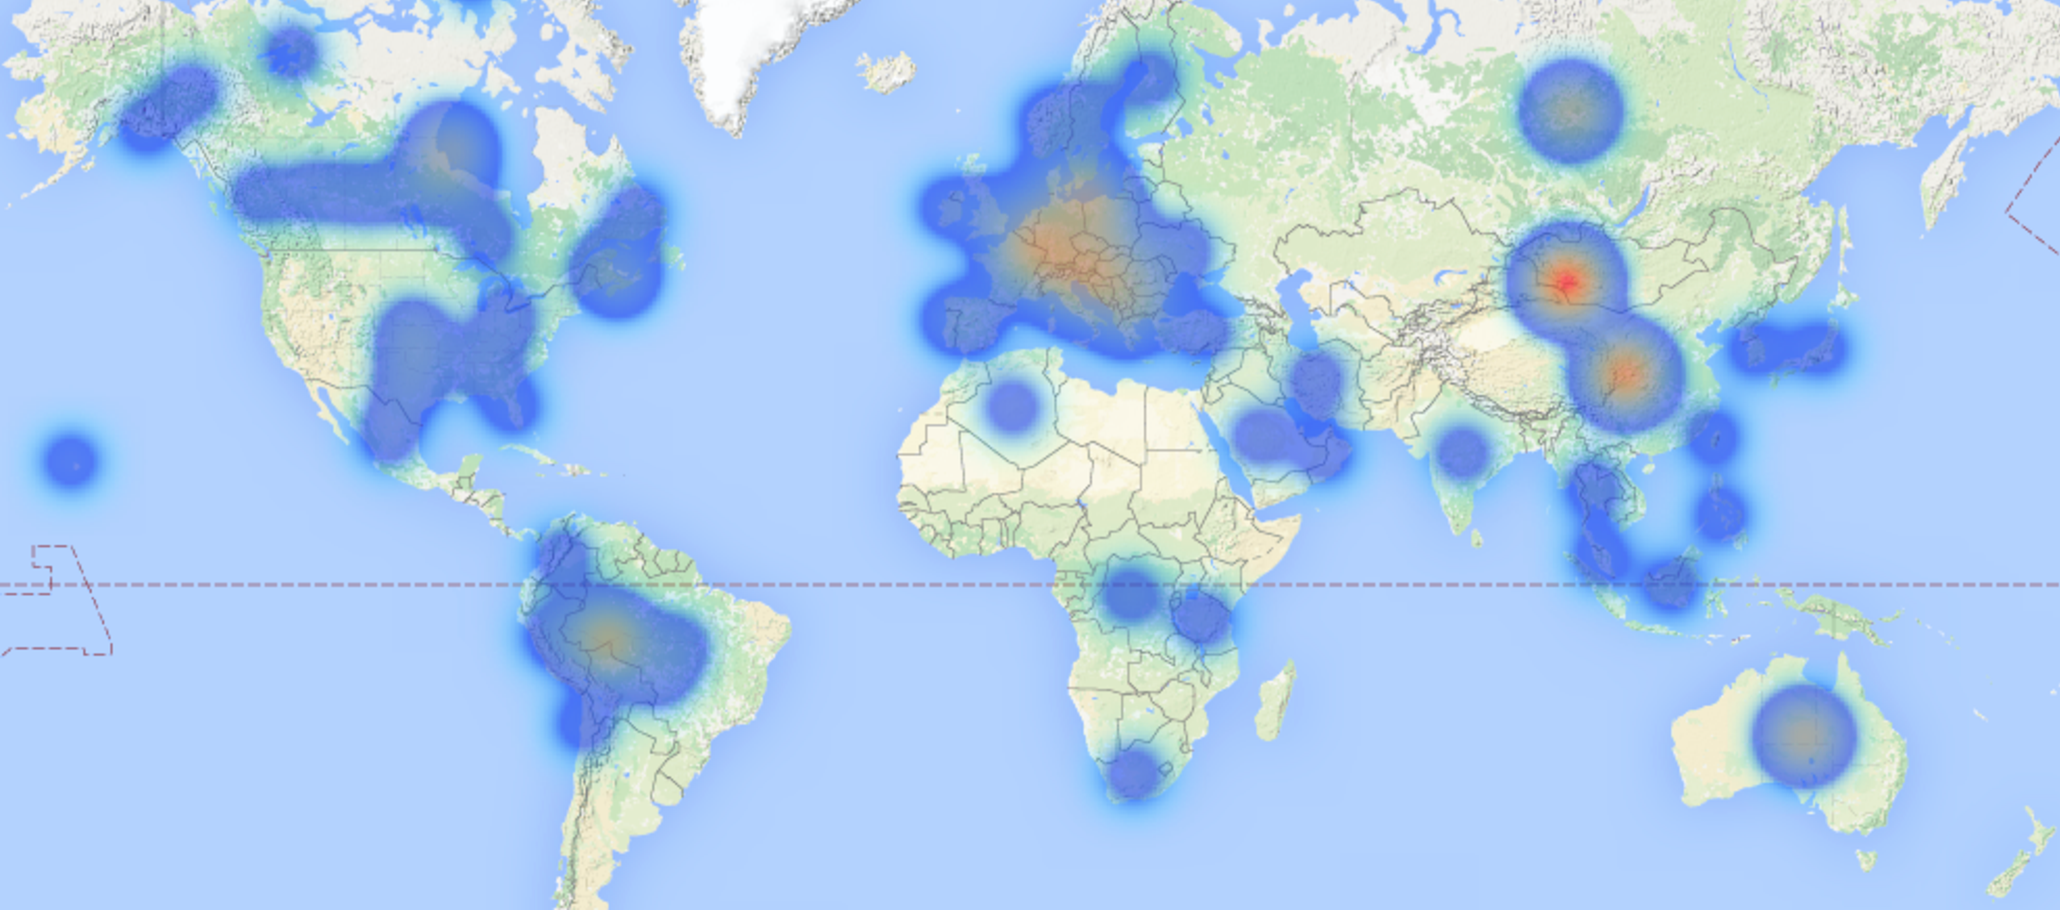
\includegraphics[width=10cm, trim= 0cm 0cm 0cm 0cm,clip]{mapacidification.pdf}
\caption{Global distribution of terrestrial acidification}
\label{fig:mapAcid}
\end{center}
\end{figure}

\subsection{Sensitivity Analysis}

The results of the sensitivity analysis is shown in Figure \ref{fig:sens}. The GWP savings from adaptive shading is dependent on the electricity mix as explained in Section \ref{ch:Meth:Opp}. Changing our assumption from the European ENTSO-E mix to a country specific mix brings interesting results. In Switzerland, the mix is dominated by hydro and nuclear power which has a very low GWP potential\cite{itten2012life}. This would then increase the emission factor of the ASF to 63.1 gCO${_2}$/kWh, which is 44\% lower than the emission factor in Switzerland. The German mix on the other hand has a higher GWP mix than the ENTSO-E mix due to their high share in coal fire plants. This then reduces the emission factor of the ASF to -792.9 gCO${_2}$/kWh.\\

The choice of actuator has a small impact on the embodied carbon emissions. Changing a single Soft Robotic Actuator (including the air compressor, tubing and maintenance) to a classical servo motor increases the embodied GWP from 2675.4 kg CO$_{2eq}$ to 3251.2 kg CO$_{2eq}$. However, the lower emissions from actuation and maintenance for servo motors cancels out this increase, resulting in an ASF with servo motors having an emission factor of -525.7 gCO${_2}$/kWh.
%\textcolor{magenta}{\textit{(Is this cited or was it also calculated? Do we provide the inventory?)}} \textcolor{red}{\textit{(Calculated, but inventory of motors needs to go in the Appendix)}}.\\

The control system design should be carefully thought out due to the high GWP of electronic components [REFERENCE REQUIRED] (value required). However limiting the individual actuation of panels to rows does not result in a significant difference. The control system required for an ASF where each panel can be independently actuated has an emission factor of -535.6 gCO${_2}$/kWh compared to the base case control system emission factor of -537.0 gCO${_2}$/kWh, where only rows are independently actuated .\\

%\textcolor{red}{The Monte Carlo Simulation did not yield any significant results / was significant. } \textcolor{blue}{Fill this out once your results come in}

% In Switzerland, we see a 6\% reduction compared to the average electricity mix. This is because the Swiss electricity mix is dominated by hydro and nuclear power which has a very low GWP potential [citation needed\textcolor{magenta}{ \textit{ecoinvent?}}]. In Germany on the other hand, the ASF has a 81\% reduction in carbon emissions as the emission factor of the electricity grid is roughly five times higher compared to Switzerland [citation needed] due to the relatively high share in coal-fired power plants.\\

\begin{figure}[H]
\begin{center}
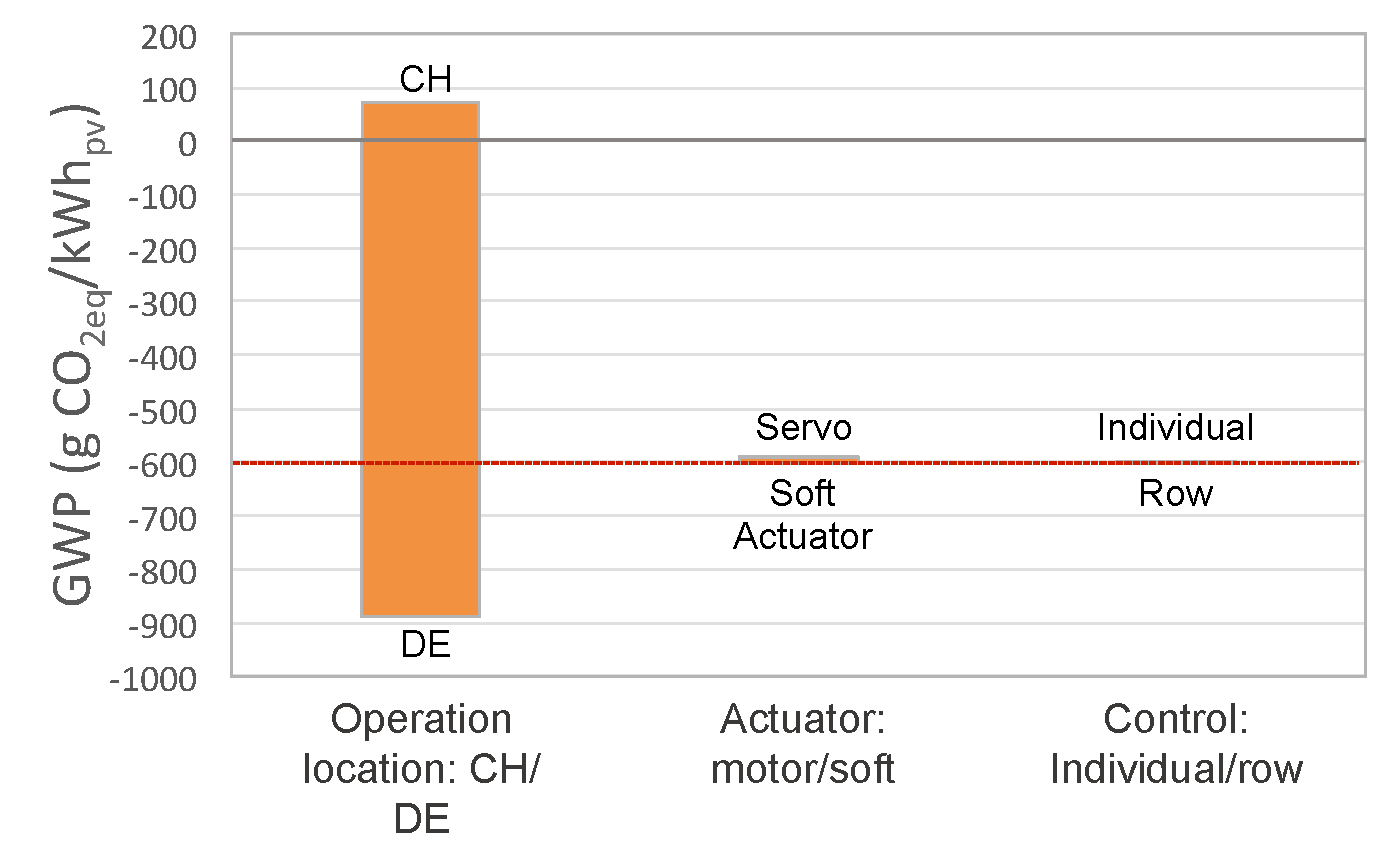
\includegraphics[width=10cm, trim= 0cm 0cm 0cm 0cm,clip]{sens.pdf}
\caption{Sensitivity analysis of the emission factor based on electricity mix, actuation system, and control system}
\label{fig:sens}
\end{center}
\end{figure}

\subsection{Comparison to existing PV technologies}

Comparison of the ASF to other PV technologies and the ENTSO-E electricity mix is highlighted in Figure \ref{fig:compPV}. Because the GWP savings through adaptive shading offsets the entire embodied GWP three-fold, we have a system that has a negative emission factor. It is this multifunctional nature of the building integrated solution that makes it superior to other technological choices. However, if the benefits of adaptive shading are not present, i.e. it is mounted on an opaque building surface, then we see reduced performance when compared to other static PV technologies. 

Figure \ref{fig:compPV} also highlights a case in Switzerland where the electricity mix has a low GWP. It is capable of out-performing Silicone based technologies but is still inferior to simply mounted CIGS panels. 

%Note that the just panels of the ASF, without the BOS, still has a higher emission factor than the CIGS installation. This is due to lower power production as a result of self shading \cite{hofer2015photovoltaics}, and situations where the panels are not optimally positioned\textcolor{magenta}{\textit{Where do these GHG figures come from?}}.

\begin{figure}[H]
\begin{center}
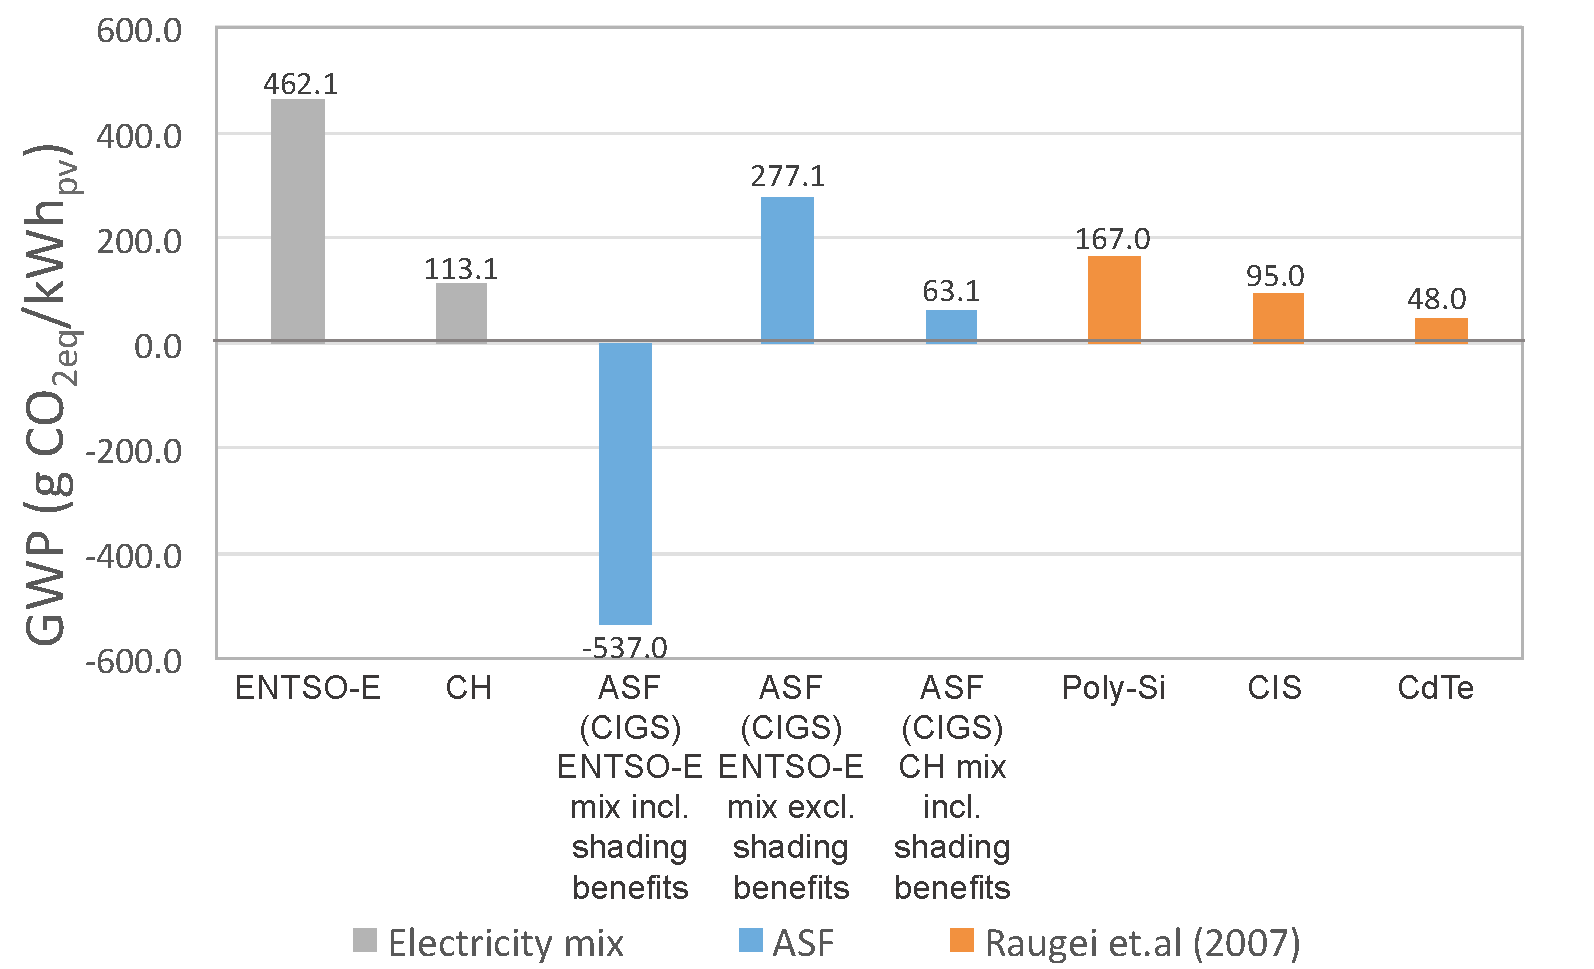
\includegraphics[width=10cm, trim= 0cm 0cm 0cm 0cm,clip]{compPV.pdf}
\caption{Comparison of thin-film and BOS to other PV technologies. I would add some extra columns, one without shading, one with the ASF in Switzerland, one with the ASF in Europe}
\label{fig:compPV}
\end{center}
\end{figure}

% \begin{figure}[H]
% \begin{center}
% 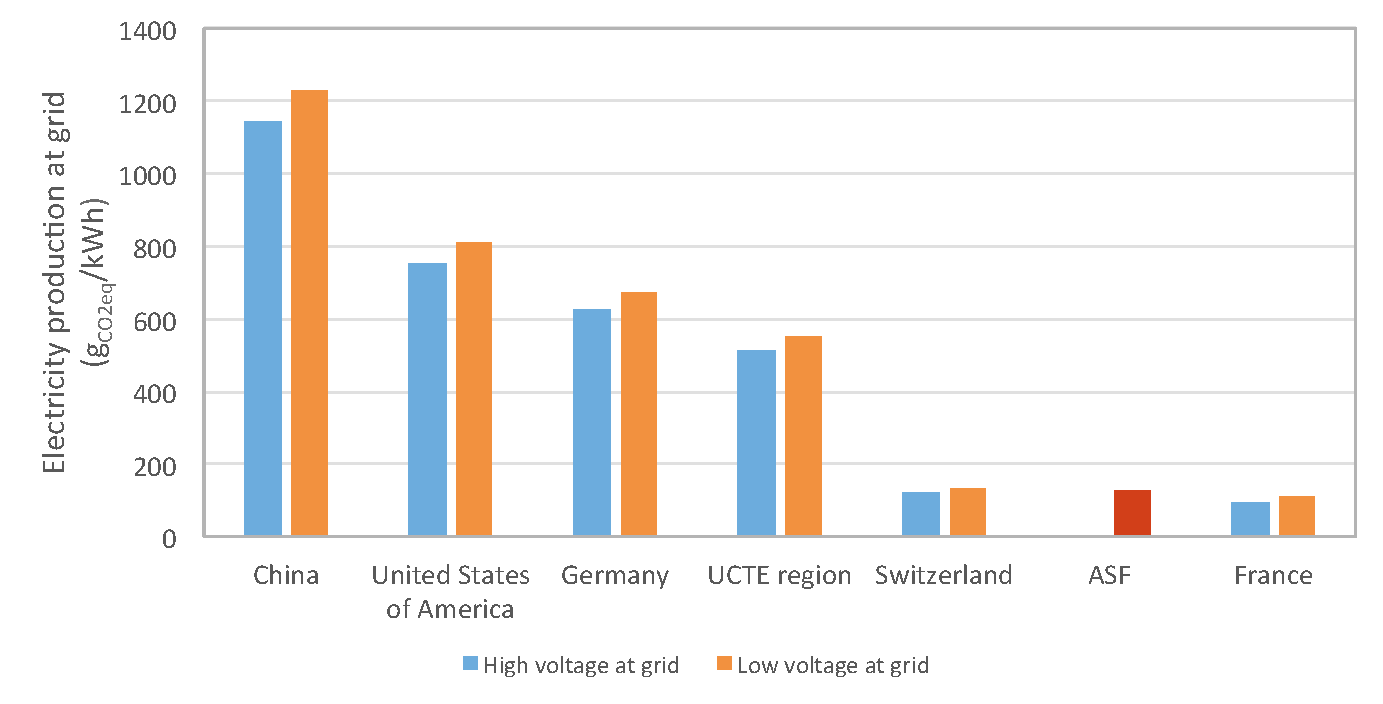
\includegraphics[width=10cm, trim= 0cm 0cm 0cm 0cm,clip]{regionGridMix.pdf}
% \caption{Comparison of the ASF when in operated in Switzerland when compared to other countries in the world that have similar climate conditions. Note that the data will have to change because we can't really compare (ASF in Switzerland) with Germany. We should be comparing the ASF in Germany with Germany}
% \label{fig:compReg}
% \end{center}
% \end{figure}



% - As input parameters of production processes are stochastic, a Monte Carlo simulation is used to include this stochastic behavior in the results, as shown in Figure \ref{fig:monte}...

% \begin{figure}[H]
% \begin{center}
% 
\includegraphics[width=10cm, trim= 0cm 0cm 0cm 0cm,clip]{monte}
% \caption{Monte carlo simulation based on input uncertainties}
% \label{fig:monte}
% \end{center}
% \end{figure}

% - Sourcing location greatly influences the embodied GWP. For photovoltaic panels, the majority of embodied emissions result from the use of electricity during production. The GWP per kwh of the Chinese electricity mix is 1145.8 ${\mathrm{gCO_2eq/kWh}}$, while in Switzerland this is only 119.6 ${\mathrm{gCO_2eq/kWh}}$.
% % cool - did we already discuss what other sensitivities to use?

% \begin{figure}[H]
% \begin{center}
% 
\includegraphics[width=10cm, trim= 0cm 0cm 0cm 0cm,clip]{sensitivity}
% \caption{Sensitivity analysis based on sourcing location}
% \label{fig:sensitivity}
% \end{center}
% \end{figure}